\documentclass[a4paper,11pt,headings=small,twocolumn]{article}

\usepackage[T1]{fontenc}
\usepackage[pdftex]{graphicx}
\usepackage{dblfloatfix}
\usepackage{multicol}
\usepackage{cite}
\usepackage{pdfpages}
\usepackage{cite}
\usepackage{tikz}
\usepackage{multirow}
\usepackage[english]{babel}
\usepackage{float}
\usepackage{mathcomp}
\graphicspath{{images/}}
\usepackage{amsmath}
\usepackage{amsfonts}
\usepackage{amssymb}
\usepackage{fouridx}
\usepackage{cancel}	
\usepackage{setspace}
\usepackage[ansinew]{inputenc}
\usepackage[format=plain,font=small,margin=10pt,labelfont=bf,labelsep=quad]{caption}
\usepackage{subcaption}
\usepackage{ipa}
\usepackage{a4wide}
\usepackage{titlesec}
\usepackage{array}
\usepackage{booktabs}
\usepackage[top=3.0cm, bottom=3.0cm, left=2cm, right=2cm]{geometry}
\sloppy
\usepackage{fancyhdr}
\usepackage{verbatim}
\usepackage{placeins}

\usepackage{hyperref}
\hypersetup{colorlinks=true}

\setlength{\columnsep}{1cm}
\DeclareMathOperator*{\argmax}{arg\,max}

\begin{comment}
NOTES/TODO

Lessons Learned:
* Covariance matrix is CRUCIAL. In fact, it's everything.
  * Should capture frames of the progression from bad to good kernel fn.
* Author was doing everything in pixels! This screws up my hyperparameters!
* How far into future to predict.
* How to get MAP (take the mean).
* Correspondence is key. In both cases, fixed major issues.
* Taking the mean to approximate the MAP: is this valid?

To Include:
* Homography transform
* Kernel & hyperparameter definition
	* Charts describing kernel
* Final MAP calculation (mean weighted by IP)
* Performance metric (path length + safety calculation)
* Final results (over how many frames? for different particle swarm sizes?)

Future:
* Do more experiments.
* Incorporate static obstacles.
* Learn how to learn my own hyperparameters.
	* Pete gave me an example script. I'd like to try learning hyperparameters for the world coordinate frame instead of doing everything in pixels.
* Tweaking of interaction potential parameters.
* Clever methods of assigning destinations to pedestrians.
* The algorithm presented here took about 2 seconds to plan a single path, with 100 particles. The original paper cites times of 0.1 seconds for the same number of particles, so there is much room for improvement here. The original paper was written in Matlab but I'm not sure the language of implementation is the bottleneck. More likely, the GPML Matlab toolbox's implementation of Gaussian processes is much more efficient than my own (some parts of the toolbox are written in C).
* Explore shared autonomy, or local vs. global path planning?
* Implement completely on-robot?

\end{comment}

\begin{document}

\twocolumn[
  \begin{@twocolumnfalse}
  \vspace{-1cm}
	\begin{flushright}
	April 10, 2014\\
	\end{flushright}
	\vspace{0.6cm}
	\LARGE{\textbf{Robot Navigation in Dense Human Crowds}\\[0.2cm] Final Report}\\\\ \\
	\large{Neil Traft\\[0.1cm] University of British Columbia}		 	 	\vspace{0.6cm}
\end{@twocolumnfalse}
]


\pagestyle{fancy}
\fancyhf{}
\fancyhead[L]{Robot Navigation in Dense Human Crowds}
\fancyhead[R]{Neil Traft --- \thepage}

\pagenumbering{arabic}
\setcounter{page}{1}
\setcounter{secnumdepth}{0}

%\onehalfspacing
\renewcommand{\thesection}{\Roman{section}}
\thispagestyle{empty}

\newcommand{\texttildemid}{{\raise.17ex\hbox{$\scriptstyle\sim$}}}
\newcommand{\f}{\mathbf{f}}
\newcommand{\fr}{\f^{(R)}}
\newcommand{\fati}{\f^{(i)}}
\newcommand{\fatj}{\f^{(j)}}
\newcommand{\samplej}{(\fatj)_i}
\newcommand{\z}{\mathbf{z}}
\newcommand{\ztot}{\z_{1:t}}
\newcommand{\pos}{\mathrm{pos}}
\newcommand{\post}{\pos^{(i)}_t}
\newcommand{\x}{\mathbf{x}}

\section{Overview}
\quad In their 2010 IROS publication \cite{Trautman2010}, Trautman and Krause develop a path planning algorithm that is safe and yet does not suffer from the ``freezing robot problem'' (FRP). Their method consists of a model of crowd interaction combined with a particle-based inference method to predict where the crowd (and the robot) should be at some time $t+1$ in the future. The idea is that if one can develop a reliable model of intelligent agents in a crowd, and include the robot as just another of those intelligent agents, then the predictions of the model yield the robot's future path.

The goal of this project is to reproduce their results in simulation on the original dataset. Given some annotated video of pedestrians in a crowd, we can choose one of the pedestrians to represent the robot, and compare the path planned by the robot to the actual path taken by the pedestrian.

\subsubsection{Interacting Gaussian Processes}
\quad The crowd interaction model is a nonparametric stochastic model based on Gaussian processes, dubbed \emph{Interacting Gaussian Processes} (IGP). In IGP, the actions of all agents, including the robot, are modeled as a joint distribution:
$$p(\fr,\f|\ztot)$$
where $\fr$ is the robot's trajectory over $T$ timesteps, $\f$ is the set of all human trajectories, and $\ztot$ is the set of all observations up to the current time point. For the purposes of this algorithm, observations of human and robot position are taken to be more or less perfect, since we are only trying to solve the navigation problem, not situational awareness.

At each timestep, each agent's new position is represented as a random variable from a probability distribution. It is important to note that this distribution is \emph{not} Gaussian, due to two major additions to avoid the uncertainty explosion which leads to the FRP (see Figure \ref{uncertainty}).

First, goal information is given as a final ``observation'' at time $T$, resulting in the full set of observations $\z_{1:t,T}$. The robot's goal, $y_T^{(R)}$, is known and can be added with good confidence. The goals of other agents can be omitted or can be added with a high variance, to encode how uncertain we are about the goal.

The second addition IGP makes to standard Gaussian processes is the inclusion of an ``interaction potential'',
\begin{align*}
\psi(\fr,\f) &= \\
\prod_{i=1}^n \prod_{j=i+1}^n \prod_{\tau=t}^T & \left( 1 - \alpha \exp\big(-\frac{1}{2h^2}|\fati_{\tau} - \fatj_{\tau}|\big) \right)
\end{align*}

In essence, this potential grows very small whenever two agents $i$ and $j$ become very close at any time $\tau$. This has the result that any set of paths where agents become too close is treated as very unlikely. The parameter $h$ controls the desired ``safety distance'' and $\alpha \in [0, 1]$ controls the ``repelling force''. Thus, the final posterior is given as:
$$ p_{IGP}(\fr,\f | \ztot) = \frac{1}{Z} \; \psi(\fr,\f) \prod_{i=1}^n p(\fati | \ztot) $$

% What is Z?
% Include image of IP?

The above is a nonlinear, multimodal distribution, so it can't be sampled directly. Instead, we sample from Gaussian priors $p(\fati|\ztot)$ and resample weighted by our desired distribution (a particle filter). This is described in the next section.

\begin{figure*}[h]
	\centering
	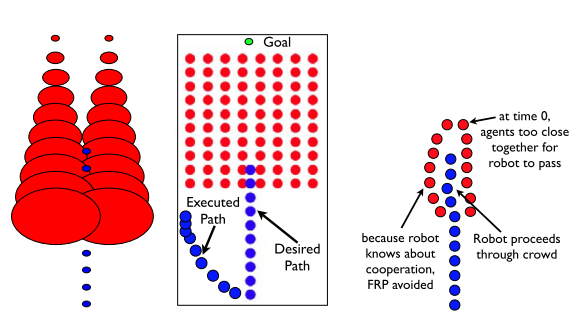
\includegraphics[width=.75\textwidth]{uncertainty-explosion.png}
	\caption{Diagrams taken from \cite{Trautman2010} describing the uncertainty explosion which leads to the Freezing Robot Problem. \textbf{Left:} Depicts the uncertainty explosion in standard motion models, where each agent's trajectory is \emph{independent} from the others. \textbf{Middle:} A demonstration of why even \emph{perfect} prediction, devoid of uncertainty, can still lead to the FRP. In crowded environments, \emph{all} paths can have a high cost function, leading to extreme evasive maneuvers or freezing. \textbf{Right:} The ideal model, based on the insight that intelligent agents engage in \emph{cooperative} collision avoidance.}
	\label{uncertainty}
\end{figure*}

\subsubsection{Importance Sampling} \label{isampling}
\quad Now that we have a model, we wish to sample from it and take the mean as the desired path. Since we can't sample from it directly, we instead use the \emph{importance sampling} technique which is widely used in particle filters. Each sample is weighted by the ratio of the IGP to the basic GP (i.e. the Gaussian distribution, without the interaction potential):
\begin{align*}
w_i &= \frac{p_{IGP}}{p_{GP}} = \frac{p_{IGP}((\fr,\f) | \ztot)}{\prod_{j=R}^n p(\samplej | \ztot)} \\
	&= \frac{\psi((\fr,\f)_i) \prod_{j=R}^n p(\samplej | \ztot)}{\prod_{j=R}^n p(\samplej | \ztot)} \\
	&= \psi((\fatj)_i)
\end{align*}
where $\samplej$ is a single sample from the trajectory of agent $j$.

Given this formulation for $p_{IGP}$ and an appropriate weighting $w_i$ for each sample, the ideal paths can now be expressed as the \emph{maximum a-posteriori} (MAP) assignment for the posterior,
$$ (\fr,\f)^* = \argmax_{\fr,\f}\left( \sum_{i=1}^N w_i(\fr,\f)_i \right) $$
where $(\fr,\f)_i$ is a set of samples from the Gaussian processes $(\fatj)_i \sim \textrm{GP}(\fatj, m_t^{(j)}, k_t^{(j)})$. The total number of samples is $N$ and we take the robot's next position to be $\fr_{t+1}$. To approximate the optimal robot path $\fr$, we take the mean path over all samples after importance resampling:
$$ \mathrm{f}^{(R)*}_t = \frac{\sum_{i=1}^N \mathrm{f}^{(R)}_t}{N} $$

\section{Implementation}
\quad The project is implemented in Python, using the OpenCV library\cite{opencv} for visualization and video playback (but not for any of the vision algorithms it provides).

\subsection{The Dataset}
\quad The dataset to be used is the ETH Walking Pedestrians (EWAP) dataset from \cite{Pellegrini2009}. It can be obtained from \cite{dataset}.

The dataset contains two annotated videos of pedestrian interaction captured from a bird's eye view. The one used depicts pedestrians entering and exiting a building.

The main annotations are a matrix where each row gives the position of an agent $i$ in a particular video frame $t$. Thus for each frame $t$ we have potentially multiple pedestrian observations $\post$, and this forms our observation at time $t$:
$$ \z_t = \pos^{(1:n)}_t $$
where one of the $n$ pedestrians is chosen to represent the robot $R$. The velocities are not used in the present IGP formulation.

The positions and velocities are in meters and were obtained with a homography matrix $H$, which is also provided with the annotations. To transform the positions back to image coordinates, it is necessary to apply the inverse homography transform:
$$ \fourIdx{m}{}{}{}\post = H_{mw}^{-1} \cdot \fourIdx{w}{}{}{}\post \quad m = \mathrm{image}, w = \mathrm{world} $$
The intrinsic camera parameters are not needed; it is presumed that they are included in the camera matrix provided by the dataset. There is also no translation needed; the origin of the world can be taken to be the (transformed) origin of the image without loss of generality. Thus, pixel coordinates can be expressed as
$$ r = -f_x \frac{x}{z} = \frac{u}{z} \qquad c = -f_y \frac{y}{z} = \frac{v}{z} $$
where $f_x,\;f_y$ are the intrinsic camera parameters and $x,\;y$ are coordinates in the image frame. So to obtain pixel coordinates from image coordinates it is necessary only to normalize so that $z=1$:
$$ \begin{pmatrix}r\\c\\1\end{pmatrix} = \begin{pmatrix}\fourIdx{m}{}{}{}x/z\\\fourIdx{m}{}{}{}y/z\\\fourIdx{m}{}{}{}z/z\end{pmatrix} $$

\subsection{Technical Hurdles}

\quad There are some nuances to using a Gaussian process that can stun and bewilder those who are new to them. IGP is very sensitive to these nuances, and an understanding of Gaussian processes is essential to getting it to work.

In addition to this, there are other parameters to be tuned and implementation choices which are left open-ended by the original author. These choices comprise the hurdles one has to clear to see good results from IGP.

\subsubsection{The Covariance Function}
\quad The covariance function (also known as a \emph{kernel}) used for the Gaussian processes in IGP is an absolutely crucial consideration. However, the authors of \cite{Trautman2010} not describe their choice of kernel. In their 2013 follow-up work, they mention the class of kernel used, but do not go into sufficient detail to reproduce their implementation. \cite{Trautman2013}

What is needed from our Gaussian process is a prior which is straight most of the time, but with some curviness. This encodes our assumptions about the way humans move. People almost always walk in straight lines, so we need a Gaussian process that gives us that. We also would like some curviness for those times when people don't walk straight, and we also need to encode the noisiness of our observations. \footnote{From correspondence with the author, Peter Trautman.}

From these requirements, we can see that the traditional kernel for Gaussian processes won't be suitable. The general-purpose kernel is the squared exponential (SE) kernel,
$$ k(\x,\x') = \sigma^2 \exp\Big(-\frac{1}{2\ell^2}|\x - \x'|^2\Big) $$
where $\x$ and $\x'$ denote two vectors of independent variables whose covariance we wish to calculate, and where $\sigma^2$ and $\ell$ are the noise and length hyperparameters, respectively.

First of all, the SE kernel is too variable; too ``curvy''. An example is given in Figure \ref{cov}. The aimlessly meandering paths seen there do not represent a person enroute to a destination. A much bigger problem, moreover, is the fact that SE is \emph{shift invariant}. Informally, this means that it will gravitate toward the mean wherever there is no data. Observe how it hovers about the origin in the example.

In contrast, the linear regression kernel is a \emph{non}-shift-invariant kernel which satisfies our need for a straight path to continue in a straight line in the absence of data. Also known as a dot product covariance function, it is expressed as
$$ k(\x,\x') = \sigma^2 + \x \cdot \x' $$

\begin{figure}[H]
	\begin{subfigure}{\linewidth}
	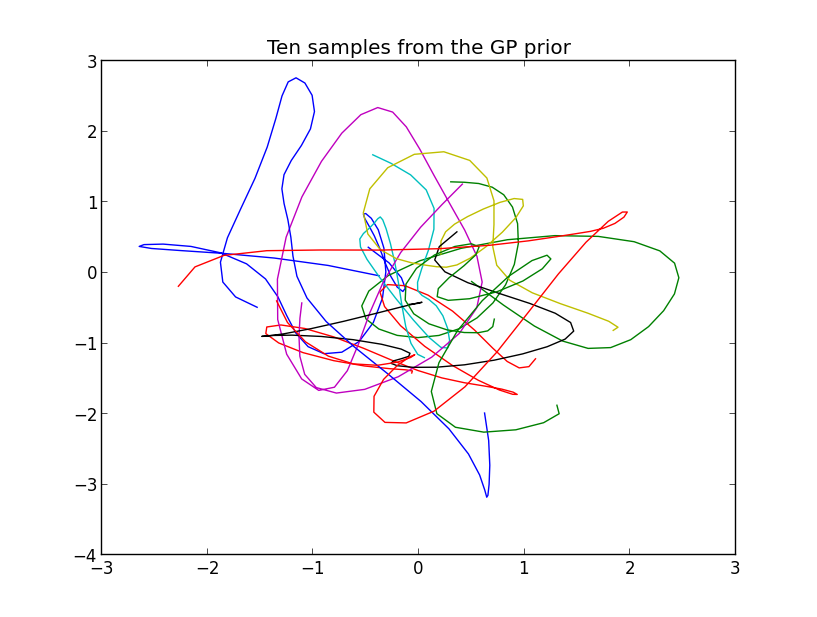
\includegraphics[width=1.0\linewidth]{SE+noise-prior.png}
	\caption{A summed kernel composed of squared exponential and noise kernels.}
	\label{a}
	\end{subfigure}
	\begin{subfigure}{\linewidth}
	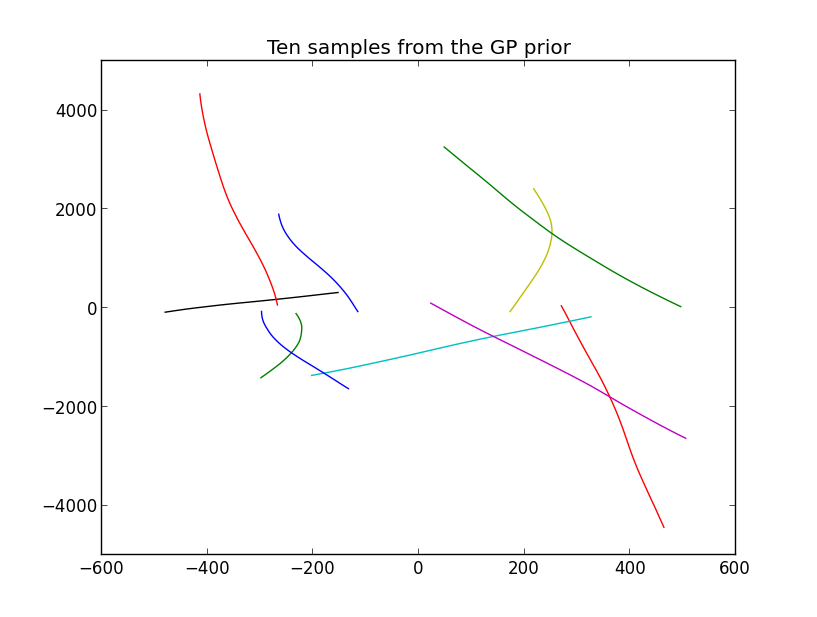
\includegraphics[width=1.0\linewidth]{matern+lin+noise-prior.png}
	\caption{A summed kernel composed of Mat�rn, linear regression, and noise kernels.}
	\label{b}
	\end{subfigure}
	\caption{The importance of choosing a proper covariance function. (\ref{a}) This is much too curvy and loopy to represent a human path. Humans generally have destinations; they don't wander aimlessly. (\ref{b}) We consider this to be a much better model of human movement. Human paths are mostly straight, but with occasional curviness.}
	\label{cov}
\end{figure}

Having only straight lines generalizes to simple linear regression, however, which is obviously not desirable. We still need to be able to approximate nonlinear paths, so we add in one of the Mat�rn class of covariance functions defined in \cite{gpml},
$$ k(r) = \left(1 + \frac{\sqrt{5}r}{\ell} + \frac{5r^2}{3\ell^2} \right) \exp\left(-\frac{\sqrt{5}r}{\ell}\right) $$
where $r = |\x-\x'|^2$. This gives us nicely shaped paths, and we finally add in a noise kernel, which is just a constant variance applied to our training data. The final choice of kernel is illustrated in Figure \ref{cov}, and an example of sampling from the posterior can be seen in Figure \ref{hp}.

\subsubsection{Kernel Hyperparameters}
\quad Perhaps equally crucial to the choice of covariance function is the choice of \emph{parameters} for the covariance function. These include such parameters as the variance $\sigma^2$ and the length-scale $\ell$. The variables are often co-dependent \footnote{Meaning that if you fix one variable, the optimal choice for the other variable depends on the value of the fixed variable} and highly dependent on the data you wish to approximate. Generally, they should be learned from the data.\cite{gpml}

I was able to obtain the original hyperparameters used for the EWAP dataset from Peter Trautman, so I did not have to learn the hyperparameters myself. Even so, producing good paths was not automatic.

Hyperparameters are directly dependent on the scale of coordinate system. This means that the hyperparameters must be tuned to the units that the data is given in. Hyperparameters learned in meters cannot be used in millimeters or image pixels: the scale of the parameters must match the scale of the data. Originally I implemented the algorithm in the world coordinate frame, and I had to switch to the image coordinate frame to match the original implementation. Figure \ref{hp} shows an exploration of the effect of hyperparameters on predicting a simple, straight-line path.

\begin{figure*}[h]
	\begin{subfigure}[b]{.5\linewidth}
	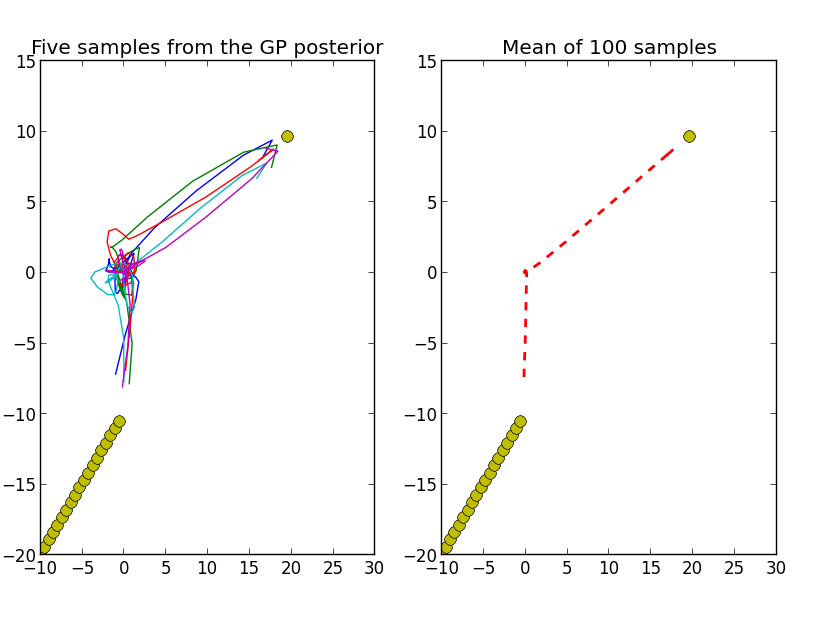
\includegraphics[width=\linewidth]{bad-cov-bad-hp.png}
	\caption{Poor choice of covariance function (squared exponential) and poorly tuned hyperparameters. Notice the attraction toward the mean, $(0,0)$.}
	\label{a}
	\end{subfigure}
	\quad
	\begin{subfigure}[b]{.5\linewidth}
	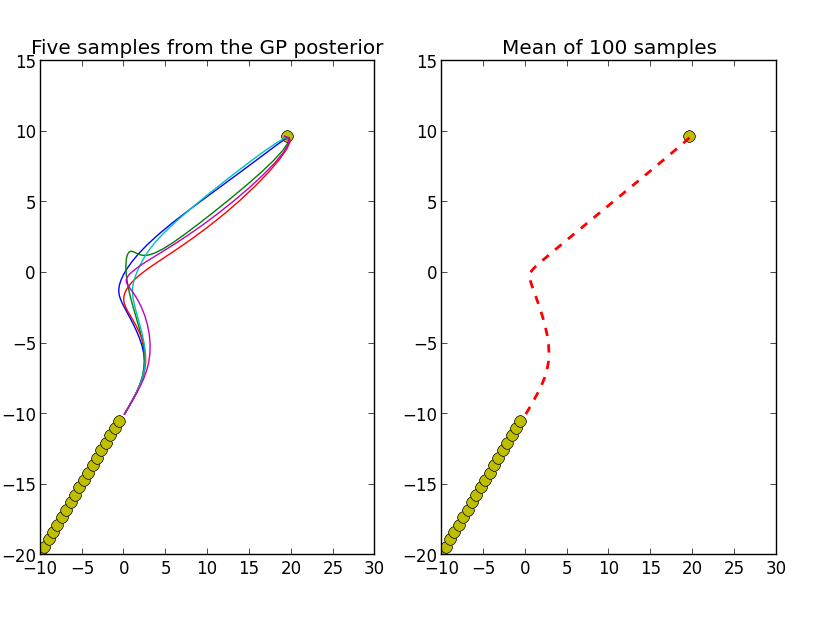
\includegraphics[width=\linewidth]{bad-cov-good-hp.png}
	\caption{Improved hyperparameters are still not enough to overcome a fundamentally incorrect covariance function.}
    \vspace{2ex}
	\label{b}
	\end{subfigure}
	\begin{subfigure}[b]{.5\linewidth}
	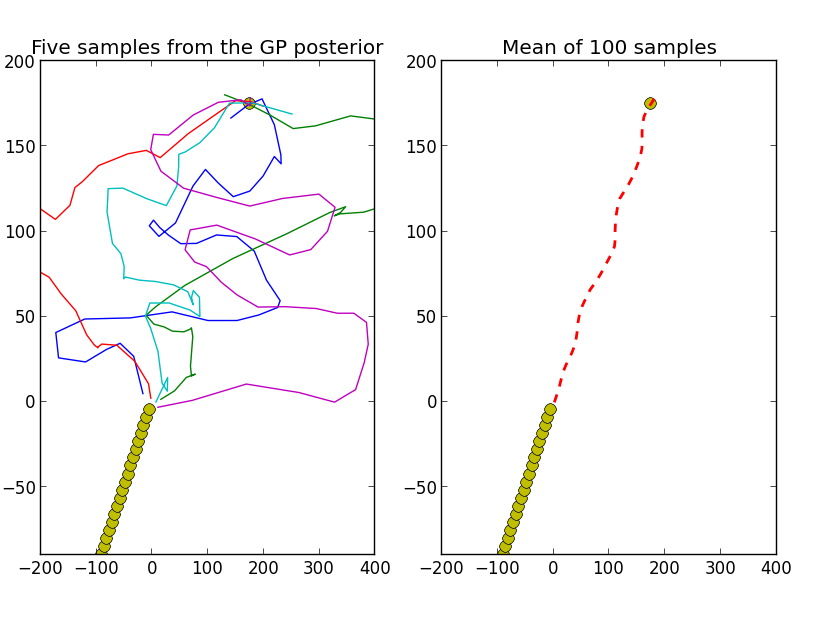
\includegraphics[width=\linewidth]{good-cov-bad-hp.png}
	\caption{Good choice of covariance function (Mat�rn + linear + noise) brings us much closer to the mark, but badly tuned hyperparameters still makes things difficult.}
	\label{c}
	\end{subfigure}
	\quad
	\begin{subfigure}[b]{.5\linewidth}
	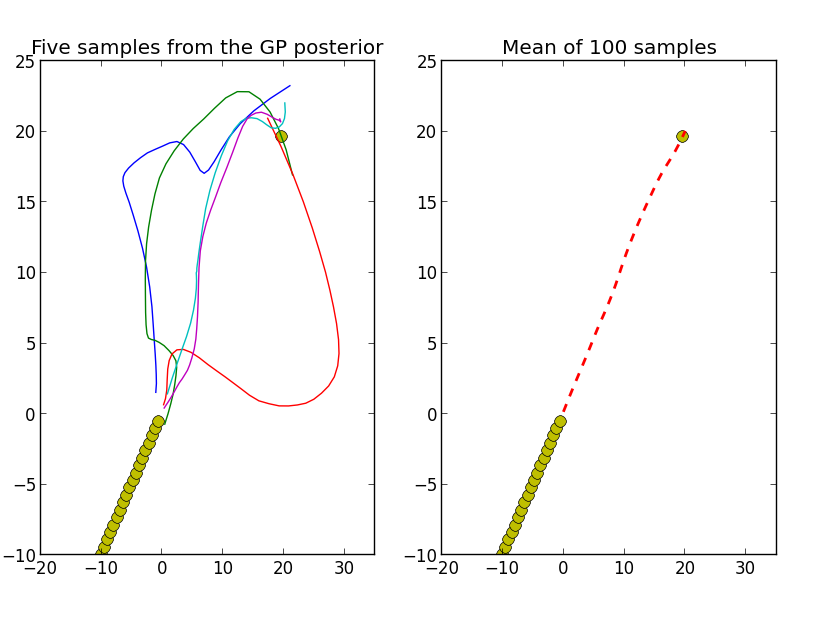
\includegraphics[width=\linewidth]{good-cov-good-hp.png}
	\caption{Good covariance function combined with good hyperparameters.}
    \vspace{2ex}
	\label{d}
	\end{subfigure}
	\caption{The importance of choosing proper hyperparameters. Hyperparameters must be learned to properly match what we expect from human and robot movement patterns. Hyperparameters must be further tuned for a particular scene, since they are closely related to the scale of our coordinate frame.}
	\label{hp}
\end{figure*}

\subsubsection{MAP Approximation}
\quad As mentioned in the \nameref{isampling} section above, the next waypoint of the robot is given by the MAP assignment of the posterior distribution. However, it is not clear how this is obtained in the original work. The answer is that we take the mean of the resampled paths in order to approximate the MAP assignment. This is roughly equivalent, therefore, of taking the weighted mean of the Gaussian process samples, prior to resampling.

Practically speaking, this is a shortcut. The reason for it is that the path with the largest weight is still unstable unless we take a very large number of samples. \footnote{This sentiment was conveyed by Peter Trautman via personal correspondence.} However, this potentially destroys multimodal distributions, which is why we used a particle filter in the first place. This seems to work well enough in this example, but an idea for improvement is described in \nameref{sec:future}.

%* Covariance matrix is CRUCIAL. In fact, it's everything.
%* Author was doing everything in pixels! This screws up my hyperparameters!
%* How far into future to predict.
%* How to get MAP (take the mean).
%* Correspondence is key. In both cases, fixed major issues.
%* Taking the mean to approximate the MAP: is this valid?

\section{Experimental Results}

\begin{figure}[h]
	\begin{subfigure}{\linewidth}
	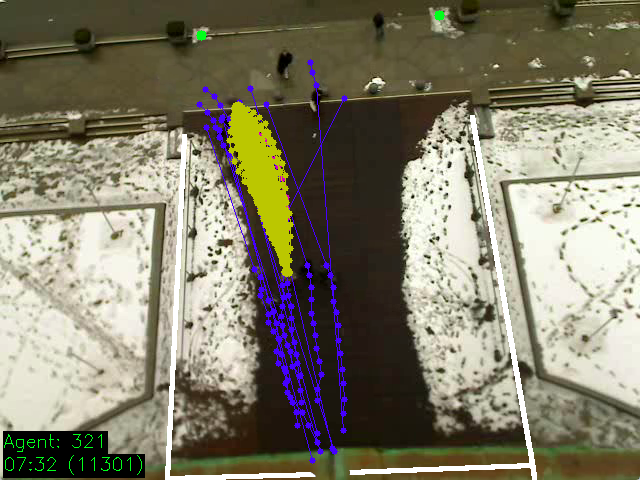
\includegraphics[width=1.0\linewidth]{screenshot-samples.png}
	\caption{The samples from the posterior distribution (after resampling according to the interaction potential).}
	\label{a}
	\end{subfigure}
	\begin{subfigure}{\linewidth}
	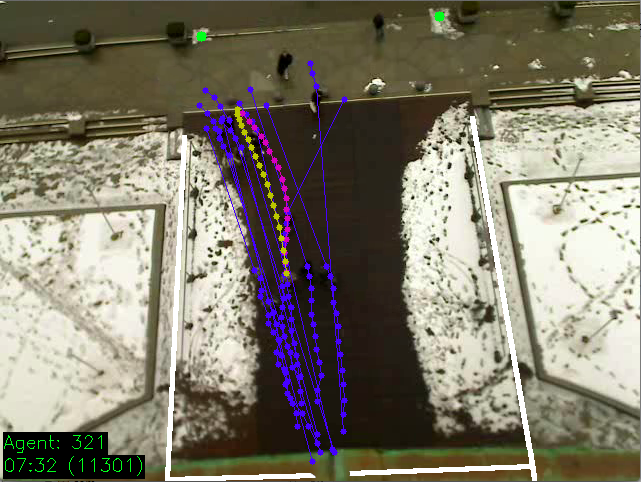
\includegraphics[width=1.0\linewidth]{screenshot-path.png}
	\caption{The path ultimately planned (yellow), compared with the pedestrian's own path (pink).}
	\label{b}
	\end{subfigure}
	\caption{Sample output of the final product. Blue paths represent each agent's path up to the current time point, as well as their ultimate destination.}
	\label{screenshot}
\end{figure}

\begin{figure}[h]
	\centering
	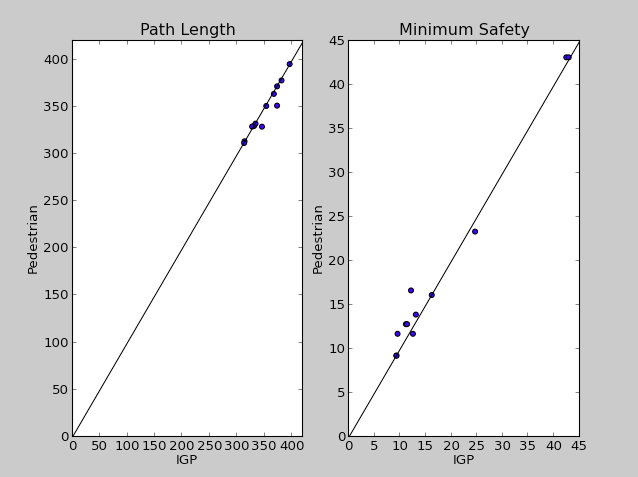
\includegraphics[width=\linewidth]{experiment.png}
	\caption{The results of the algorithm performed on 12 pedestrians from a particularly crowded segment of the video. Observe that IGP almost always finds an equal length or shorter path than the pedestrian. However, the pedestrian usually maintains a larger distance from other agents, though IGP never goes below the lowest observed actual separation (\texttildemid10 pixels), so it is considered safe.}
	\label{experiment}
\end{figure}

\begin{figure}[h]
	\centering
	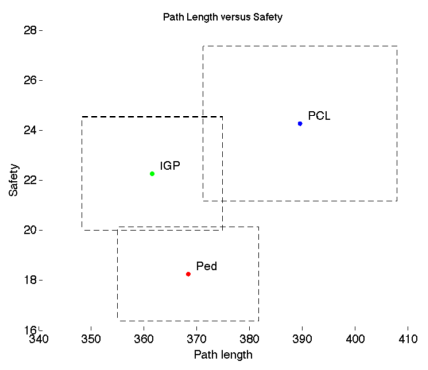
\includegraphics[width=\linewidth]{sample-results.png}
	\caption{The results reported in the original paper, compiled from 10 trials. Here, we see that IGP outperforms human pedestrians in both path length and path safety. We aren't told which 10 pedestrians are evaluated in the original paper, so these results are somewhat anecdotal and will not necessarily align with our own.}
	\label{sample}
\end{figure}


\section{Next Steps} \label{sec:future}


\section{Conclusion}
\quad In this project I have demonstrated the feasibility of the Interacting Gaussian Processes algorithm for path planning through human crowds. From these preliminary experiments, it seems that IGP has potential as a tractable method for searching through an infinitely large state space of actions.

However, there is more work to be done. I was not able to match the author's reported performance, neither in path planning nor in computational efficiency. I have noted some immediate improvements that could be made to my implementation which would likely close this gap. Still, I've also demonstrated IGP's fragility in terms of its heavy reliance on parameter tuning. A compelling research problem for the future would be to create a version of IGP which learns these parameters online.


\bibliography{references}
\bibliographystyle{ieeetr}

\end{document}
